%<dscrpt>Introduction aux fonctions d'une variable complexe. Théorème de Rouché</dscrpt>
Ce texte fait intervenir des fonctions $\mathcal{C}^{\infty}(\R)$, périodiques de période $2\pi$ et à valeurs dans $\C$. De telles fonctions sont appelées des \emph{lacets}. Un lacet $\gamma$ peut être vu comme un mouvement. Pour $t\in \R$, le complexe $\gamma(t)$ représente la position dans le plan d'un point mobile. La trajectoire (notée $\Gamma$) est l'ensemble des points par où est passé le mobile. \`A cause de la périodicité,
\[
 \Gamma = \left\lbrace \gamma(t), \; t\in \R \right\rbrace = \left\lbrace \gamma(t), \; t\in [0, 2\pi] \right\rbrace .
\]
Les figures \ref{fig: Eindice_1} et \ref{fig: Eindice_2} présentent les trajectoires $\Gamma$ pour deux lacets.
\begin{figure}[h]
  \centering
  \subfloat[$\gamma(t) = e^{it}$.\label{fig: Eindice_1}]{
    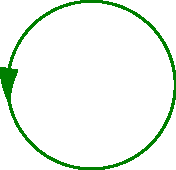
\includegraphics{./Eindice_1.pdf}
  }
  \hspace{3cm}
  \subfloat[$\gamma(t)= e^{2it} - e^{it} -1$.\label{fig: Eindice_2}]{
    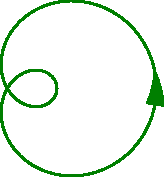
\includegraphics{./Eindice_2.pdf}
  }
  \caption{Exemples de trajectoires.}
\end{figure}

Pour un lacet $\gamma$ et un complexe $z\notin \Gamma$, \emph{l'indice} de $z$ par rapport à $\gamma$ est 
\[
 I_\gamma (z) = \frac{1}{2 i \pi}\int_{0}^{2\pi}\frac{\gamma'(t)}{\gamma(t) - z} \, dt.
\]
Il s'agit de l'intégrale d'une fonction d'une variable réelle $\mathcal{C}^{\infty}$ à valeurs complexes où $\gamma'(t)$ est la notation habituelle pour la dérivée de $\gamma$. Pour un nombre complexe $z$ tel que $|z|\neq 1$, on note $I_0(z)$ son indice par rapport au mouvement circulaire.
\[
 I_0(z) = \frac{1}{2  \pi}\int_{0}^{2\pi}\frac{ e^{it}}{e^{it} - z} \, dt\hspace{0.5cm} \text{avec } \gamma(t) = e^{it}.
\]

\subsection*{Partie préliminaire.}
\begin{enumerate}
 \item Soit $f$ continue dans $\R$, périodique de période $T>0$ et à valeurs complexes.\newline
Montrer que la fonction de $\R$ dans $\C$, $ x \mapsto \int_x^{x+T}f(t)\, dt$ est constante.

 \item Montrer que:
\[
 \forall x \in \R^*, \; \arctan x + \arctan \frac{1}{x} =
 \left\lbrace 
 \begin{aligned}
  \frac{\pi}{2} &\text{ si } x > 0 \\
  -\frac{\pi}{2} &\text{ si } x < 0
 \end{aligned}
 \right. .
\]

 \item Pour $\theta$ entre $0$ et $\frac{\pi}{2}$, exprimer $\cos \theta$ en fonction de $\tan \frac{\theta}{2}$.
\end{enumerate}

\subsection*{Partie I. Calcul direct de $I_0(z)$.}
Dans cette partie, $z \in \C$, $|z|\neq 1$ et $\varphi\in \R$ est un argument de $z$. On note
\[
 A(z) = \Re(I_0(z)), \hspace{1cm} B(z) = \Im(I_0(z)).
\]
\begin{enumerate}
 \item Soit $r \in \R \setminus\left\lbrace -1, +1 \right\rbrace$. En effectuant le changement de variable $t = \tan \frac{\theta}{2}$, montrer
\[
 \int_0^{\frac{\pi}{2}}\frac{d\theta}{1+r^2 - 2r\cos \theta}
 =
 \frac{2}{1-r^2}\arctan\left( \frac{1 + r}{1 - r}\right) .
\]

 \item 
 \begin{enumerate}
  \item  Montrer que
\[
 A(z) = \frac{1}{2\pi}\int_{0}^{2\pi}\frac{1 - |z| \cos(t-\varphi)}{1 + |z|^2 - 2|z|\cos(t-\varphi)}\, dt, \hspace{0.5cm}
 B(z) = 0.
\]
  \item Montrer que 
\[
 I_0(z) = \frac{1}{2} + 
 \frac{1-|z|^2}{4\pi}
 \int_0^{2\pi}\frac{dt}{1 + |z|^2 - 2|z|\cos(t-\varphi)}.
\]
 \end{enumerate}

  \item Montrer que
\begin{multline*}
 \int_0^{2\pi}\frac{dt}{1 + |z|^2 - 2|z|\cos(t-\varphi)} = \\
 2\left( 
 \int_0^{\frac{\pi}{2}}\frac{d\theta}{1 + |z|^2 - 2|z|\cos \theta}
 +
 \int_0^{\frac{\pi}{2}}\frac{d\theta}{1 + |z|^2 + 2|z|\cos \theta}
 \right) .
\end{multline*}
En déduire
$
I_0(z)=
\left\lbrace 
\begin{aligned}
 1 &\text{ si } |z| < 1\\
 0 &\text{ si } |z| > 1
\end{aligned}
\right. 
$.
\end{enumerate}

\subsection*{Partie II. L'indice est un entier.}
On revient au cas général: $\gamma$ est un lacet et $z \in \C \setminus \Gamma$ n'est pas sur la trajectoire.
On considère l'équation différentielle
\begin{equation*}
 (\gamma - z) y' - \gamma' y = 0
\end{equation*}
où la fonction inconnue $y$ est à valeurs complexes.
\begin{enumerate}
 \item Déterminer la solution évidente qui prend en $t=0$ la valeur $\gamma(0) - z$.
 \item En utilisant un résultat de cours cité précisément, exprimer cette solution avec la fonction exponentielle complexe et une intégrale.
 \item Montrer que $I_\gamma(z) \in \Z$.
\end{enumerate}

